\documentclass{sig-alternate-05-2015}


% http://tex.stackexchange.com/questions/117816/using-us-letter-within-an-acm-paper
\pdfpagewidth=8.5in
\pdfpageheight=11in


\def\sharedaffiliation{
\end{tabular}
\begin{tabular}{c}}

\begin{document}




\setcopyright{rightsretained}

% DOI
\doi{http://dx.doi.org/10.1145/3029798.3038320}

% ISBN
\isbn{978-1-4503-4336-7/17/03}

%Conference
\conferenceinfo{HRI '17,}{March 6--9, 2017, Vienna, Austria.}

\clubpenalty=10000 
\widowpenalty = 10000



\title{Towards the Quantification of Human-Robot Imitation Using Wearable Inertial Sensors}


\numberofauthors{3} 

\author{
\alignauthor Miguel P. Xochicale\\
      \email{map479@bham.ac.uk}
\alignauthor Chris Baber\\
      \email{c.baber@bham.ac.uk}
      \sharedaffiliation
      \affaddr{School of Electronic, Electrical and Systems Engineering}  \\
      \affaddr{The University of Birmingham}   \\
      \affaddr{Birmingham, B15 2TT, UK}
}     
      

\maketitle
\begin{abstract}
In this study, we propose a metric in order to quantify how closely a healthy participant imitates a robot,
for which we use inertial sensors attached to both individual participant and to a humanoid-robot.
For the experiment, twelve healthy participants were invited to perform 
simple arm movements in order to apply
the state space reconstruction which 
is based on the method of time-delay embedding and PCA.
Although the performed arm movements of the healthy participants were very simple,
the study reveals that the participants showed different ranges of the proposed metric 
that can be linked to the level of imitation.
Such a metric can be improved in order to determine
a detailed scoring of human-robot imitation
during training or rehabilitation activities.
\end{abstract}



\begin{CCSXML}
<ccs2012>
<concept>
<concept_id>10010520.10010553.10010554.10010558</concept_id>
<concept_desc>Computer systems organization~External interfaces for robotics</concept_desc>
<concept_significance>500</concept_significance>
</concept>
<concept>
<concept_id>10010520.10010553.10010554.10010555</concept_id>
<concept_desc>Computer systems organization~Robotic components</concept_desc>
<concept_significance>300</concept_significance>
</concept>
</ccs2012>
\end{CCSXML}

\ccsdesc[500]{Computer systems organization~External interfaces for robotics}
\ccsdesc[300]{Computer systems organization~Robotic components}



\printccsdesc

\keywords{Human-robot Imitation, Movement Variability, Wearable Inertial Sensors,
Non-linear Dynamics, State Space Reconstruction}

\section{Introduction}
Recently, NAO, a humanoid robot, has successfully been used both as a fitness coach for the elderly 
and as an instructor of rehabilitation for children.
For instance, G{\"{o}}rer et al. \cite{Gorer2016} used NAO as an exercise tutor and an Asus Xtion RGB-D camera 
which were employed to extract the joint angles of a human demonstrator and some participants. 
Absolute differences of the joint angles between the human demonstrator and the participants
were used to create a corrective feedback for the movement of the elderly 
with respect to (i) speed adjustment, (ii) amplitude adjustment, (iii) mirroring detection, and (iv) motion.
However, when participants are seated, the RGB-D camera cannot provide 
correct skeletal information of the participant.
There is also room for implementation of a detailed scoring system for the human-robot imitation
since the score is only based on how well the participant follows the verbal commands of the robot.
Similarly, Guneysu et al. \cite{Guneysu2015} used NAO and wearable inertial sensors
to monitor the motions of arm rehabilitation of children.
The challenge for Guneysu et al. was to keep the children motivated in order to imitate 
movements for arm rehabilitation therapy. 
For this, NAO successfully captured the attention of the children,
while the use of inertial sensors were ideal to avoid any  
obstructions between the children, the therapist and the robot.
However, as part of their study, 
it was revealed that the four physiotherapists all moved in slightly different ways
while performing arm motions; 
which is reflected in the differences of frequency and amplitude of the movements
as well as in the initial positions of their hands.

For this study, we are therefore proposing a framework based on the state space reconstruction 
in order to explore a metric that can help us to determine 
how close the participants mimic the original movement of the robot.
We also use inertial sensors to avoid any obstructions during the interaction 
and NAO to control simple movements that participants have to imitate.

\section{METHODS}

\subsection{Research Question}

How to analyse  data collected from wearable inertial sensors attached both 
to a person and to a humanoid robot in order to quantify how closely a participant 
imitates a robot.


\subsection{Participants}
Twelve right-handed healthy participants (two females and ten males)
with a mean age of 19.5$\pm$0.79 (from now on abbreviated as p01 to p12) were invited to 
participate in this study. 
All participants provided informed consent forms prior to participation.
The design of the experiment was approved by the University of Birmingham's ethics approval
process. 

 
\subsection{Procedure}
Participants were asked to imitate horizontal and vertical arm movements
performed by NAO.
Such simple movements were repeated ten times for both the participant and the robot
 in a front to front imitation activity
and
 wearable inertial sensors were attached to the right hand of the participant and to the left hand of the robot
(Figure~\ref{fig:main}A).
Data were then collected at a sampling rate of 50Hz with two NeMEMSi inertial sensors
which provide the tri-axial data of the accelerometer, gyroscope and magnetometer sensors and
quaternions \cite{Comotti2014}. 
It is important to note that due to the 2-page limit, we only present
results for the horizontal movement and focus our analysis on the $z$ axis from the gyroscope sensor ($g_z$) 
which is mostly affected by the nature of the horizontal movement (Figure~\ref{fig:main}A).


\section{State Space reconstruction}

The state space reconstruction (SSR) is based on the methods of time-delay embedding and PCA \cite{Gibson1992}.
Our motivation to use the method of time-delay embedding
is due to the non-linear structure of the time-series
which is 
presented 
as
different periods and amplitudes of the time-series 
between repetitions of movements and across movements of participants (Figure~\ref{fig:main}B and \ref{fig:main}C).
The method of time-delay embedding is an array of 
delayed copies of the available time series $x(n)$ and is defined as  
$ \overline{x}(n) = \{  x(n), x(n-\tau), x(n-2\tau), \dots,x(n-(m-1)\tau)\}$;
where $m$ is the embedding dimension and $\tau$ is the delay embedding.
PCA is used as a method for dimensionality reduction due to its non-parametric features.
PCA is therefore applied to $ \overline{x}(n)$ in order to get $PC_1, PC_2, \dots, PC_m$ 
to which we use $PC_1$ and $PC_2$ 
to create a state space reconstruction (Figure~\ref{fig:main}D, \ref{fig:main}E, and \ref{fig:main}F).
Finally, we computed euclidean distances in the state space 
from (0,0) point to each ($PC_1(i),PC_2(i)$) point where $1 \leq i \leq m$
in order to obtain the box-and-whisker plots for each participant (Figure~\ref{fig:main}G).


\section{PRELIMINARY RESULTS}

The robot's performance was highly consistent 
as indicated by the orange line in time-series in Figure~\ref{fig:main}B and \ref{fig:main}C,
and by the tight circular shape in the state space in Figure~\ref{fig:main}D.
Compared with the consistency of the robot, 
p01 was able to imitate the robot's movement well by maintained a good level of consistency
as shown both 
by the blue line in Figure~\ref{fig:main}B and 
by the circular shape in Figure~\ref{fig:main}E.
The other participant here, p05, had some problems in following the robot.
This is shown by the blue line in 
Figure~\ref{fig:main}C and the disjointed circular shape 
of the  state space in Figure~\ref{fig:main}F.
Such shapes in the  state space are linked either 
to a maximum interquartile range
or 
to a minimum interquartile range of the respective box-and-whisker plot (Figure~\ref{fig:main}G).
Therefore, one  can see that participants p02, p05, p07, and p12 seemed
to have more difficulty than others in maintaining a consistent response
to the robot's movement.


\begin{figure}[ht]
\centering
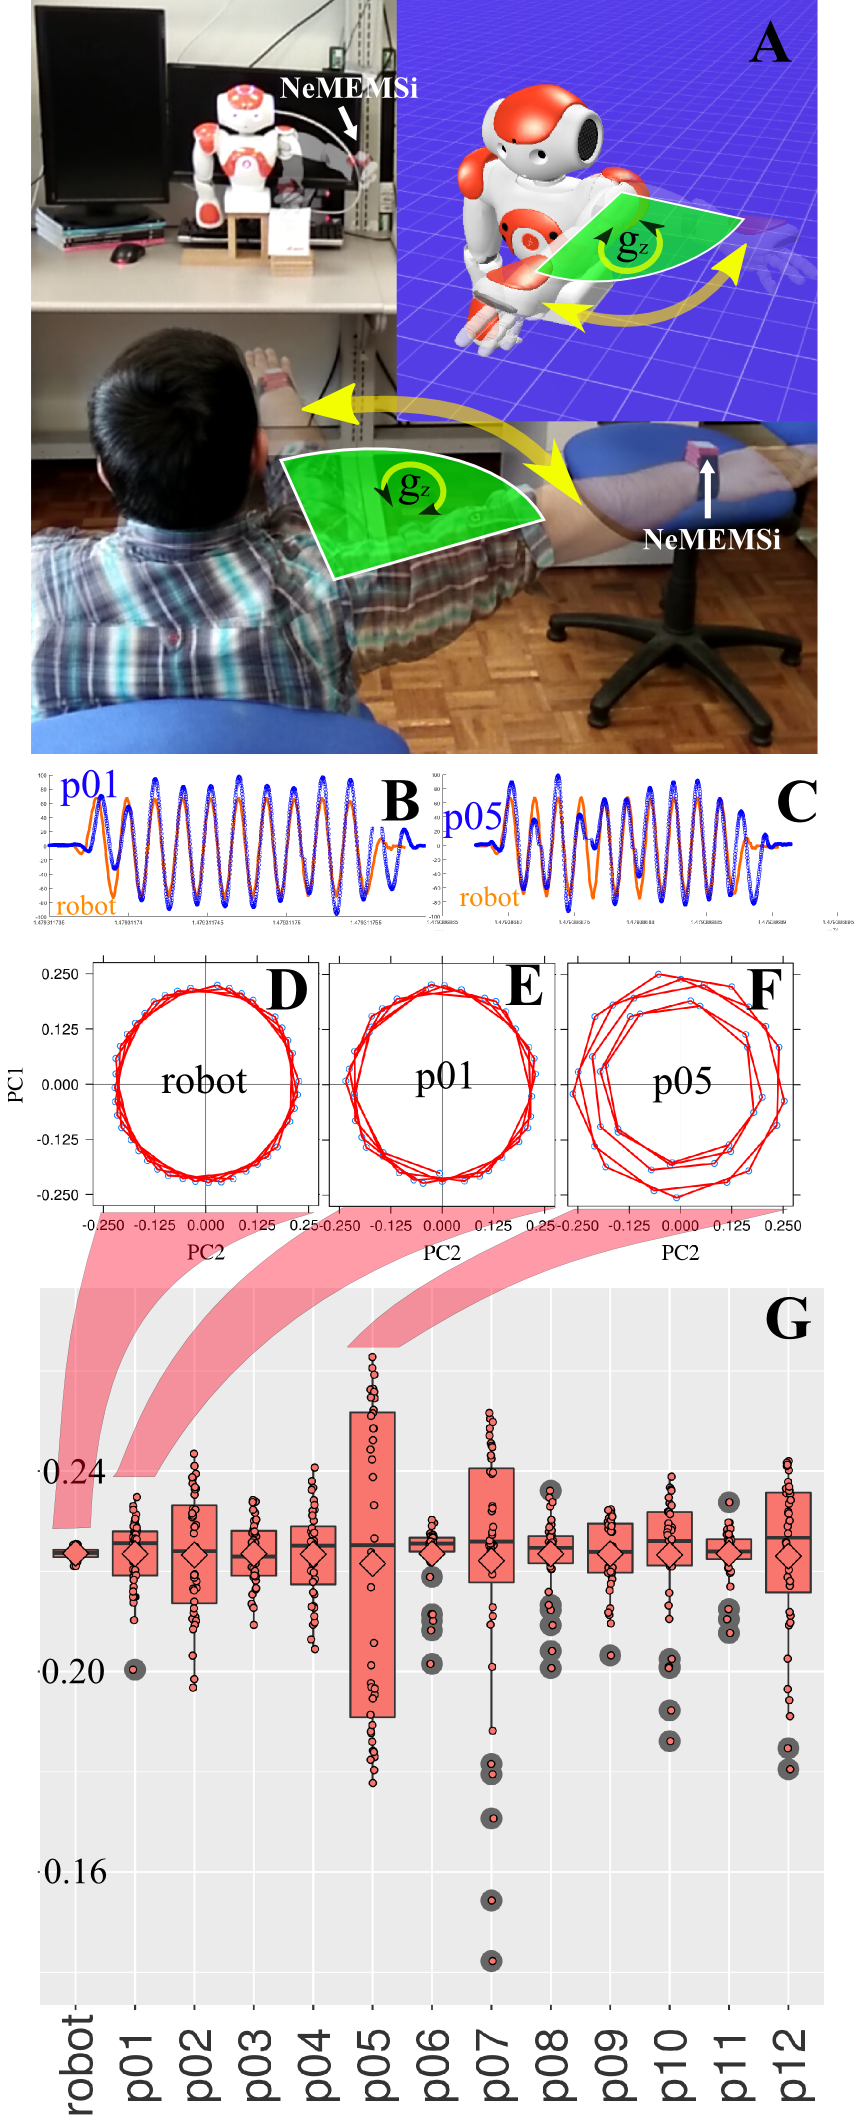
\includegraphics[width=0.245\textwidth]{fig06}
\caption{
Horizontal movement performed by both NAO and participant 05 (A). 
Smoothed angular acceleration $g_z$ for participant 01  and robot (B)
and for participant 05 and robot (C).
Reconstructed state spaces  ($m=40$, $\tau=10$) for robot (D), participant 01 (E), and participant 05 (F).
Euclidean distances from the state space for the robot and twelve participants (G).
}
\label{fig:main}
\end{figure}



\section{CONCLUSIONS AND FUTURE WORK}
We proposed a metric to quantify how closely a participant can imitate a robot for simple arm
movements.
It can be noted
that participants show different ranges 
of imitation which can be linked to a scoring system of human-robot imitation.
However, the quality of such metric is debatable and needs further investigation.

For future research, there are four areas that we intend to investigate:
(i) data collection from a wider range of individuals (differing gender, age and state of health)
and from additional inertial sensors attached to the body;
(ii) exploration of complex movements which can be performed by both persons and NAO;
(iii) undertake a wider review of non-linear techniques that can be used for 
the assessment of human-robot imitation; and, 
(iv) exploration of convolutional neural networks for automatic 
classification of the levels of human-robot imitation.



\bibliographystyle{abbrv}
\bibliography{literature} 

\end{document}